%!TEX root = ../main.tex

Στο παρών κεφάλαιο θα πραγματοποιηθεί μια αναλυτική παρουσίαση του θεωρητικού και τεχνολογικού υπόβαθρου, που αποτέλεσε βάση για την υλοποίηση της εφαρμογής. Αρχικά, θα δοθεί μια εξήγηση για το τι εστί απώλεια όρασης, τι δυσκολίες αντιμετωπίζουν τα άτομα με αυτό το είδος αναπηρίας, καθώς και τις τρέχουσες λύσεις για την καταπολέμηση δυσκολιών προσβασιμότητας (\hyperref[sec:visualImpairment]{Κεφάλαιο~\ref*{sec:visualImpairment}}). Στη συνέχεια, θα δοθεί ο ορισμός της εκτεταμένης πραγματικότητας, καθώς και τις εφαρμογές που βρίσκει στην καθημερινότητα του ανθρώπου (\hyperref[sec:extendedReality]{Κεφάλαιο~\ref*{sec:extendedReality}}). Τέλος, θα δοθεί μια περιγραφή της συσκευής Microsoft Hololens 2 και των λειτουργιών της (\hyperref[sec:hololensDesc]{Κεφάλαιο~\ref*{sec:hololensDesc}}), και τα εργαλεία, τα οποία θα χρησιμοποιηθούν για την ανάπτυξη της εφαρμογής (\hyperref[sec:hololensTools]{Κεφάλαιο~\ref*{sec:hololensTools}}).

\section{Όραση}\label{sec:visualImpairment}
\subsection{Τρόπος Λειτουργίας}\label{subsec:visionDefinition}
Η όραση αποτελεί μία από τις βασικές αισθήσεις του ανθρώπου. Η αίσθηση αυτή βασίζεται στη λειτουργία του ματιού, το οποίο αποτελεί το αισθητήριο όργανο και στο εσωτερικό του οποίου εισέρχεται το φως, διαπερνώντας αρχικά το κερατωειδή χιτώνα και την κόρη και προσπίπτει, τελικά, στον αμφιβληστροειδή χιτώνα (\hyperref[fig:eye_anatomy]{\schema~\ref*{fig:eye_anatomy}}). Αυτό οδηγεί σε διέγερση των οπτικών νεύρων και τα οπτικά σήματα, που αποστέλλονται στον εγκέφαλο, μετατρέπονται σε εικόνα~\cite{nationaleyeinstitute_2022_how}\cite{anspaugh_2022_vision}.

\begin{figure}[!h]
  \centering
  \includegraphics[width=90mm]{images/eye_anatomy.jpg}
  \caption[Η ανατομία του ματιού]{Η ανατομία του ματιού {\footnotesize(Πηγή: dreamstime.com)}}\label{fig:eye_anatomy}
\end{figure}

\subsection{Απώλεια Όρασης: Κατηγοροποίηση και Αιτίες}\label{subsec:visionCauses}
Όταν η φυσιολογική λειτουργία του αισθητήριου οργάνου διαταραχθεί, τότε το άτομο έρχεται αντιμέτωπο με κάποιο τύπο προβλήματος όρασης. Με βάση τον Παγκόσμιο Οργανισμό Υγείας (Π.Ο.Υ.), τα άτομα αυτά κατηγοροποιούνται σε 6 κατηγορίες (Κατηγορία 0 έως Κατηγορία 5), ανάλογα την οπτική τους οξύτητα, δηλαδή την ικανότητά τους να διακρίνουν σχήματα και λεπτομέρειες από κάποια δεδομένη απόσταση:
\begin{itemize}
    \item Στην κατηγορία 0 ανήκουν άτομα με με πλήρως ή σχεδόν πλήρως λειτουργική όραση
    \item Στην κατηγορία 1 και 2 ανήκουν άτομα που έχουν υποστεί μερική απώλεια της όρασής τους
    \item Τέλος, στις κατηγορίες 3, 4 και 5 εντάσσονται τα άτομα με σχεδόν πλήρη ή πλήρη απώλεια όρασης
\end{itemize}
Αντιθέτως, για κοντινές αποστάσεις, τα άτομα με προβλήματα όρασης εντάσσονται σε μία μόνο κατηγορία~\cite{worldhealthorganization_2019_world}.

Οι κυριότερες αιτίες, οι οποίες προκαλούν προβλήματα όρασης, αποτελούν:
\begin{itemize}
    \item τα διαθλαστικά σφάλματα
    \item ο καταρράκτης
    \item η διαβητική αμφιβληστροειδοπάθεια
    \item το γλαύκωμα
    \item η ηλικιακή εκφύλιση της ωχράς κηλίδας
\end{itemize}
Από τα ανωτέρω, η κυριότερη αίτια πλήρης απώλειας όρασης σε άτομα ηλικίας 50 ετών και άνω αποτελεί ο καταρράκτης, σε ποσοστό 46\% των ατόμων που υπέστησαν πλήρη απώλεια όρασης το 2020. Αντιθέτως, για την ίδια ηλικιακή ομάδα, η οποία αντιμετώπιζε μερική απώλεια όρασης, κύριες αιτίες αποτελούν τα υποδιορθωμένα διαθλαστικά σφάλματα και ο καταρράκτης, σε ποσοστό 30\% το καθένα για το ίδιο έτος~\cite{adelson_2021_causes}.

\subsection{Απώλεια Όρασης: Αντίκτυπος}\label{subsec:visionImpact}
Η απώλεια όρασης έχει ιδιαίτερο αντίκτυπο στην προσωπική, κοινωνική και οικονομική ζωή του ατόμου, ανεξάρτητα της ηλικίας του. Η εκπλήρωση απλών καθημερινών εργασιών μπορεί να αποδειχθεί ιδιαίτερα δύσκολη και χρονοβόρα, επιδεινώνοντας ιδιαίτερα την ποιότητα ζωής του ατόμου~\cite{west_2002_how}\cite{khorraminejad_2016_the}, ακόμη και σε επίπεδο χαμηλότερο από αυτό ατόμων που αντιμετωπίζουν χρόνια νοσήματα~\cite{langelaan_2007_impact}.



Η εμφάνιση προβλημάτων όρασης σε αρκετά νεαρή ηλικία μπορεί να επηρεάσει αισθητά την ανάπτυξη ικανοτήτων, όπως είναι η κινητήρια και η γνωστική ικανότητα και η κοινωνική καλλιέργεια~\cite{worldhealthorganization_2023_blindness}. Αντιθέτως, στην ενήλικη ζωή του ατόμου, μπορεί να δυσκολέψει την εύρεση εργασίας και να επηρεάσει την ψυχική του υγεία, προκαλώντας μέχρι και άγχος και κατάθλιψη~\cite{khorraminejad_2016_the}. Τέλος, σε άτομα αρκετά μεγάλης ηλικίας, η απώλεια όρασης μπορεί να αποτελέσει τροχοπέδη για βασικές λειτουργίες, όπως είναι το περπατήμα με εγγενές κίνδυνο την πτώση και τον τραυματισμό~\cite{worldhealthorganization_2023_blindness}.

\subsection{Απώλεια Όρασης: Λύσεις}\label{subsec:visionSolutions}
Πλήθος λύσεων είναι διαθέσιμες στο μέσο άνθρωπο, οι οποίες στοχεύουν στην πρόληψη της απώλειας της όρασης ή στην επιδιόρθωση αυτής. Σε απλές περιπττώσεις, όπως είναι η μυωπία, πρεσβυωπία, κ.λ.π., το πρόβλημα μπορεί να επιλυθεί με χρήση διορθωτικών φακών ή εγχείρηση στο αισθητήριο όργανο~\cite{worldhealthorganization_2023_blindness}. Επίσης, για άτομα που δεν μπορούν να επιδιορθώσουν το πρόβλημα όρασής τους, έχουν αναπτυχθεί συσκευές και τεχνολογίες, οι οποίες συνεχώς εξελίσσονται και έχουν ως σκοπό την εξυπηρέτηση του ατόμου σε διάφορες πτυχές της καθημερινότητάς του. Επί δεκαετείες, το μπαστούνι αποτελεί μια αρκετά διαδεδομένη συσκευή, που βοηθά ένα άτομο να αναγνωρίζει εμπόδια, καθώς περιηγείται σε έναν χώρο. Σε συνδυασμό με την απτική πλακόστρωση (\hyperref[fig:tactile_paving]{\schema~\ref*{fig:tactile_paving}}), το άτομο μπορεί να περιηγηθεί σε δημόσιο χώρο, όντας συνεχώς ενήμερο για την ύπαρξη εμποδίων, όπως δρόμοι, διάβαση πεζών, γραμμές τραμ, στη διαδρομή του, ανάλογα με το μοτίβο των πλακών του πεζοδρομίου~\cite{mashiata_2022_towards}.
\begin{figure}[!h]
  \centering
  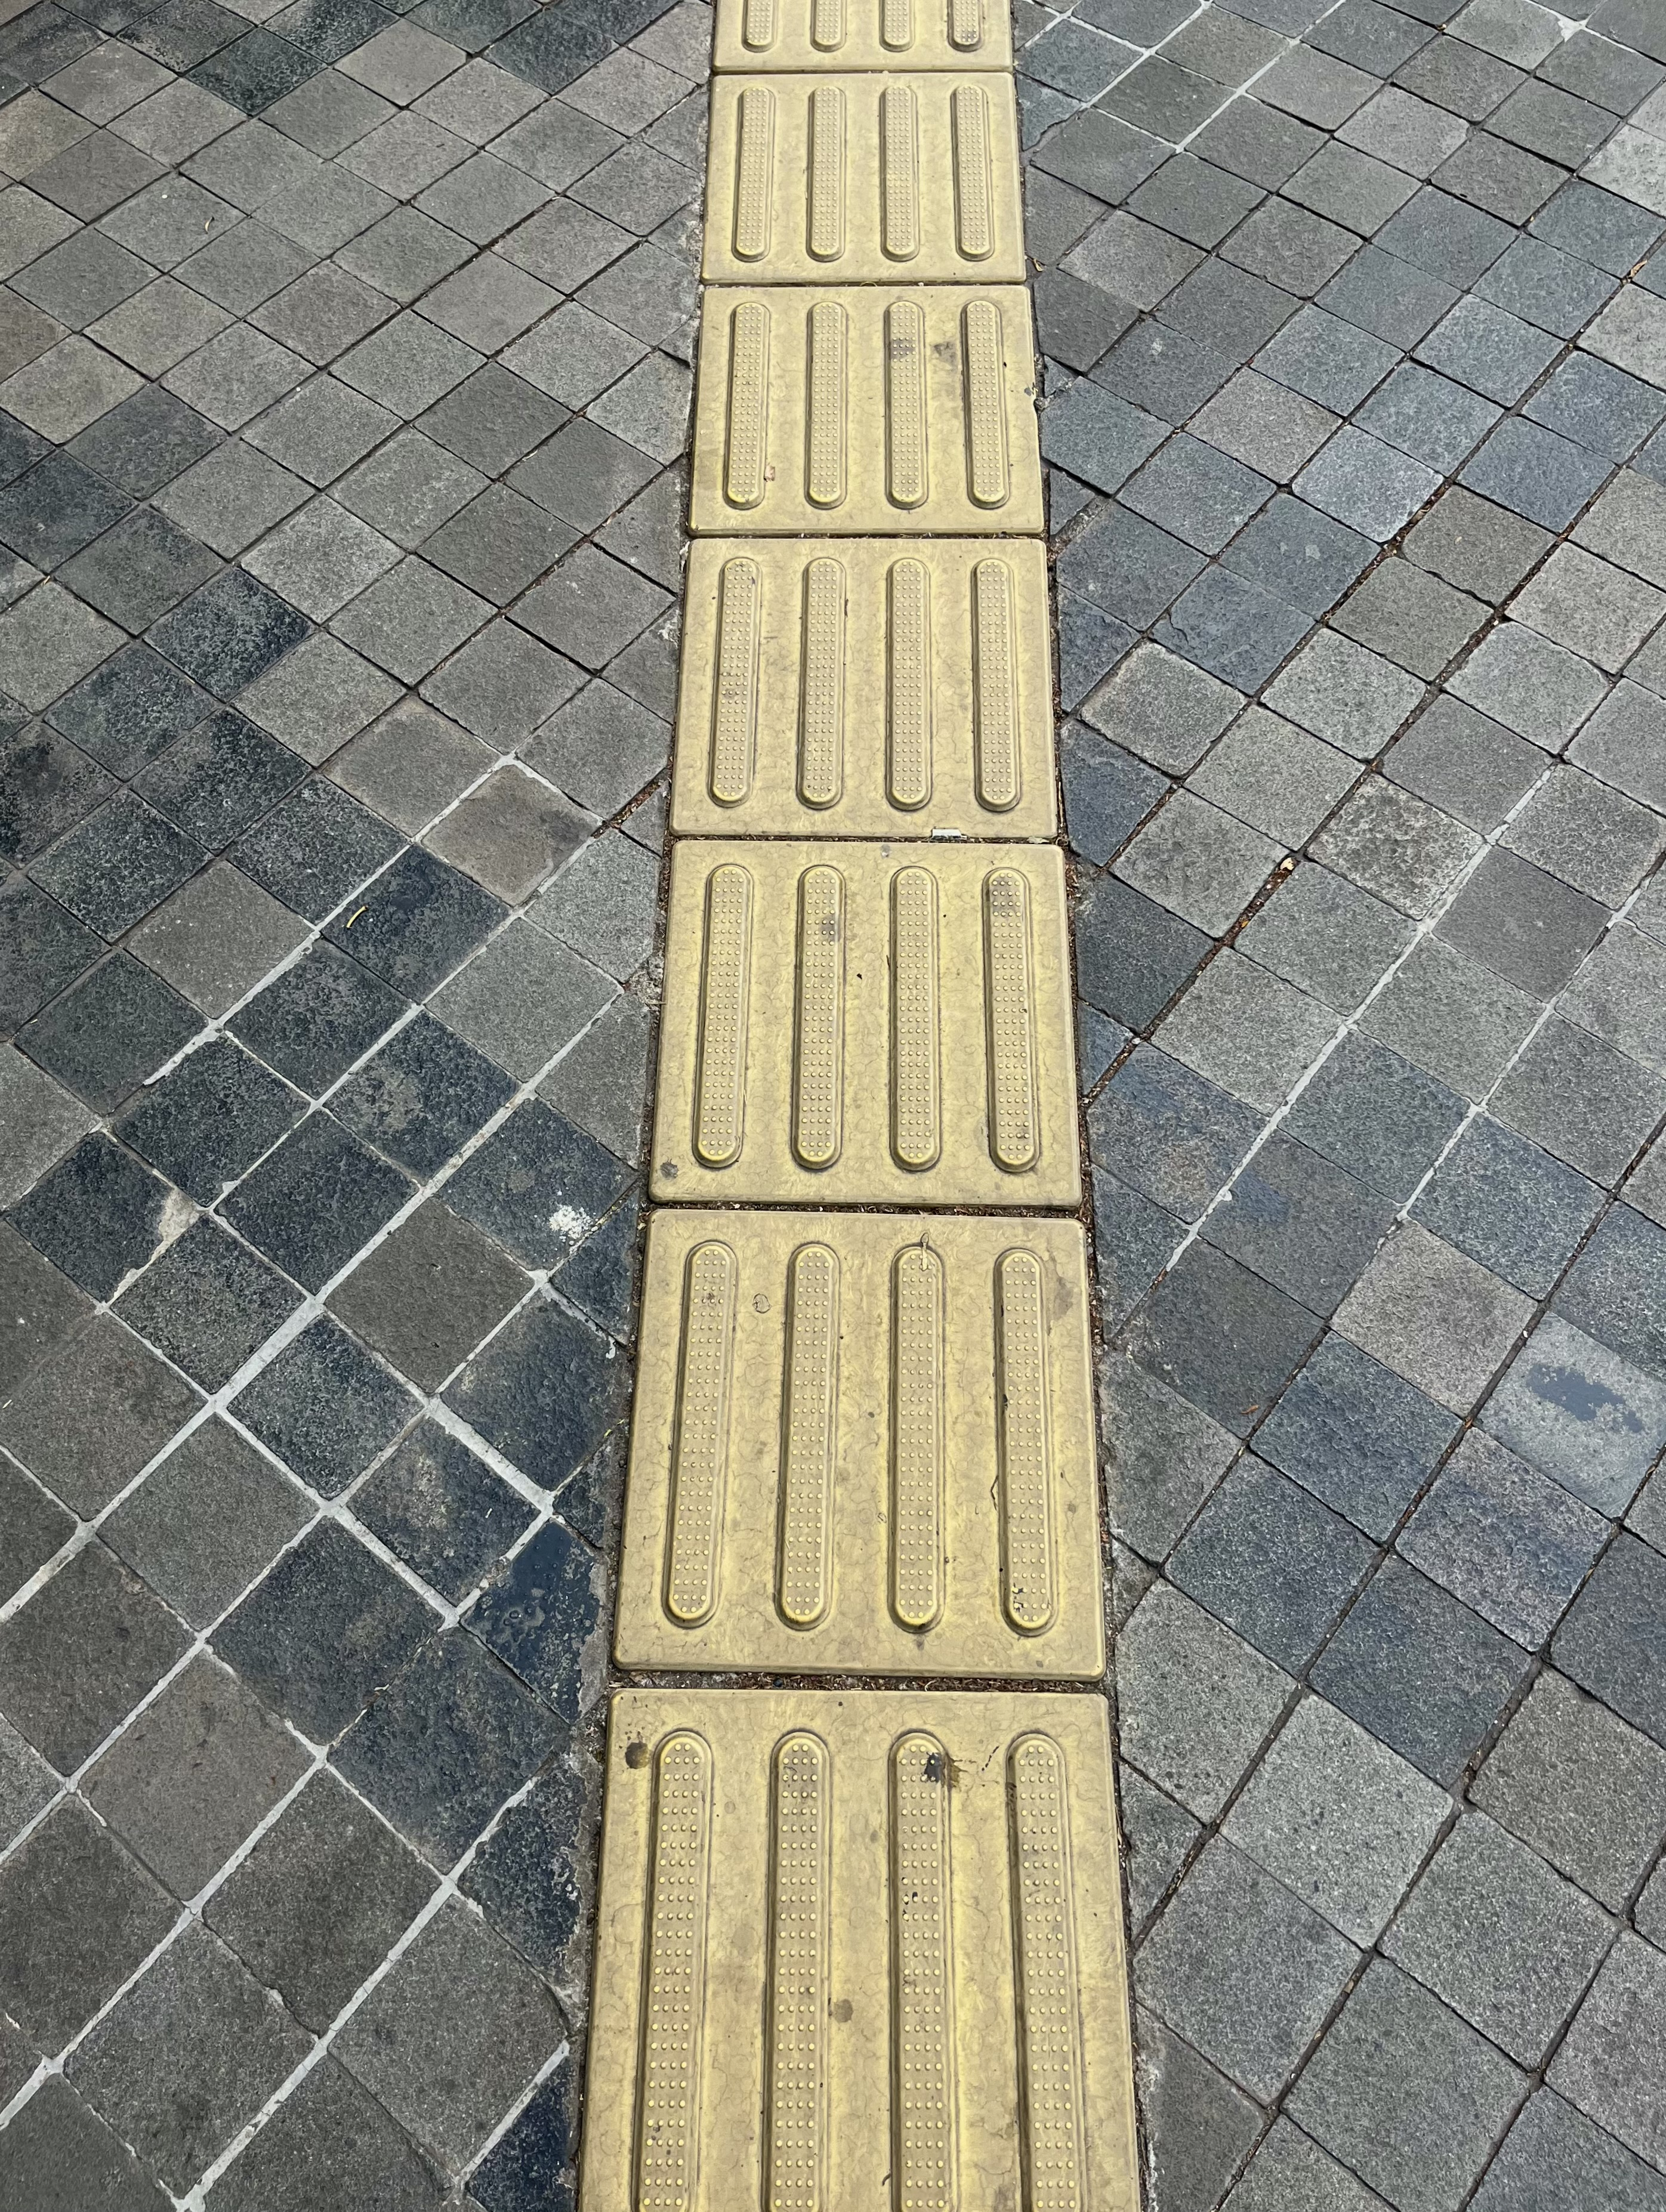
\includegraphics[width=60mm]{images/tactile-paving.jpg}
  \caption[Απτική πλακόστρωση]{Απτική πλακόστρωση {\footnotesize(Πηγή: vecteezy.com)}}\label{fig:tactile_paving}
\end{figure}\\
Ευρέως διαδεδομένη είναι και η χρήση σκύλων-βοηθών, οι οποίοι είναι ειδικά εκπαιδευμένοι σχετικά με την αναπηρία του ιδιοκτήτη τους με σκοπό να τους εξυπηρετήσουν στις ιδιαίτερες ανάγκες που μπορεί να έχουν. Στην περίπτωση των ατόμων με προβλήματα όρασης, σκοπός τους είναι να κατευθύνουν τον ιδιοκτήτη τους στο προορισμό του, ειδοποιώντας τον για πιθανά εμπόδια~\cite{illinoisuniversitylibrary_2013_libguides}. Τέλος, αναπτύχθηκε το σύστημα γραφής Braille, ώστε να είναι εφικτή η ανάγνωση κειμένων με τη βοήθεια της αφής.

Στη σύγχρονη εποχή, όλο και περισσότερες συσκευές κατασκευάζονται λαμβάνοντας εκ των προτέρων υπόψη τη δυνατότητα χρήσης αυτών από άτομα με περιορισμένη όραση. Οι κινητές συσκευές διαθέτουν λογισμικό screen reader (π.χ. TalkBack σε Android συσκεύες ή VoiceOver σε iOS συσκευές), διευκολύνοντας την πλοήγηση του χρήστη στις εφαρμογές του κινητού, καθώς πραγματοποιούν καταγραφή και αναγνώριση των κειμένων και των λειτουργιών, που βρίσκονται στην οθόνη τη δεδομένη χρονική στιγμή, και ο χρήστης, με συγκεκριμένες χειρονομίες, επιλέγει αν επιθυμεί την ανάγνωση κάποιου κειμένου με χρήση text-to-speech ή την πραγματοποίηση κάποιας ενέργειας~\cite{americanfoundationfortheblind_2019_screen}. Επιπλέον, η γλώσσα προγραμματισμού HTML δίνει τη δυνανότητα στους προγραμματιστές να κατασκευάσουν ιστοσελίδες, οι οποίες θα είναι προσβάσιμες από άτομα με περιορισμένη όραση, καθώς οι screen readers θα μπορούν να αναγνωρίζουν τμήματα της ιστοσελίδας, όπως επικεφαλίδες, υπερσυνδέσμους, κουμπιά και το σκοπό που επιτελούν~\cite{w3schools_2020_html}.

Όσον αφορά την περιήγηση ατόμων σε ανοιχτούς ή κλειστούς χώρους, πληθώρα συσκευών έχουν κατασκευαστεί, οι οποίες βελτιώνουν ήδη υπάρχουσες ή προσφέρουν έναν εναλλακτικό τρόπο λειτουργίας και παροχής βοήθειας. Παραδείγματα τέτοιων συσκευών αποτελούν:
\begin{itemize}
  \item \textbf{biped}: Συσκευή, η οποία φοριέται γύρω από το λαιμό του χρήστη. Διαθέτει 3 κάμερες, που προσφέρουν πεδίο ορατότητας 170\textdegree, και ενσωματώνουν λογισμικό για τον εντοπισμό και αναγνώριση εμποδίων. Ο χρήστης προειδοποιείται για εμπόδια με μια ηχητική προειδοποίηση.~\cite{biped}
  \item \textbf{OrCam MyEye}: Φορητή συσκευή, η οποία προσφέρει τη δυνατότητα ανάγνωσης κειμένων, αναγνώρισης αντικειμένων, χρωμάτων και προσώπων.~\cite{ghebali_2023_orcam}
  \item \textbf{BlindSquare}: Εφαρμογή πλοήγησης, η οποία παρέχει αναλύτικες\\οδηγίες στο χρήστη, ώστε να κατευθυνθεί στο προορισμό του, παρέχοντας παράλληλα πληροφορίες για το περιβάλλον του και για σημεία ενδιαφέροντος.~\cite{blindsquare}
  \item \textbf{Be My Eyes}: Εφαρμογή, η οποία επιτρέπει σε χρήστες να έρθουν σε επικοινωνία με εθελοντές μέσω βιντεοκλήσης, με σκοπό να ζητήσουν βοήθεια.~\cite{a2019_be}
  \item \textbf{WeWALK}: Αποτελεί ένα εξάρτημα για μπαστούνια, το οποίο έχει τη δυνατότητα να εντοπίζει εμπόδια σε χαμηλό ύψος με χρήση υπερήχων και να ειδοποιεί το χρήστη με δονήσεις και ήχο.~\cite{wewalk}
  \item \textbf{Seeing AI}: Εφαρμογή της Microsoft, η οποία, με χρήση τεχνητής νοημοσύνης, παρέχει περιγραφές των αντικειμένων, χρωμάτων, ανθρώπων και κειμένων, τα οποία στοχεύει ο χρήστης με την κάμερα του κινητού του τηλεφώνου.~\cite{seeing}
\end{itemize}

%=========================================

\section{Εκτεταμένη Πραγματικότητα}\label{sec:extendedReality}
% chktex-file 8

\tolerance=10000 Η εκτεταμένη πραγματικότητα (Extended Reality - XR) αποτελεί μια ιδιαιτέρως ευρεία έννοια, η οποία χρησιμοποιήθηκε πρώτη φορά το 1991 από τους Steve Mann και Charles Wyckoff, κατά την προσπάθεια κατασκευής συσκευών εικονικής/επαυξημένης πραγματικότητας~\cite{mann_2023_fundamentals}\cite{mann_1991_extended}. Αποτελεί `ομπρέλα' εννοιών και περιλαμβάνεις τις έννοιες της Εικονικής (Virtual Reality - VR, \hyperref[subsec:mixedReality]{Κεφάλαιο~\ref*{subsec:mixedReality}}), της Επαυξημένης (Augmented Reality - AR, \hyperref[subsec:augmentedReality]{Κεφάλαιο~\ref*{subsec:augmentedReality}}) και της Μικτής Πραγματικότητας (Mixed Reality - MR, \hyperref[subsec:mixedReality]{Κεφάλαιο~\ref*{subsec:mixedReality}})~\cite{milgram_1994_augmented}. To 1994, οι Paul Milgram και Fumio Kishino όρισαν ένα συνεχές μεταξύ πραγματικού και εικονικού κόσμου (\hyperref[fig:rv_continuum]{\schema~\ref*{fig:rv_continuum}}). Αυτοί οι δύο κόσμοι αποτελούν τα άκρα της κλίμακας και μεταξύ αυτών υπάρχουν οι έννοιες της επαυξημένης και μικτής πραγματικότητας, καθώς και της επαυξημένης εικονικότητας.
\begin{figure}[!h]
    \centering
    \includegraphics[width=120mm]{images/rv_continuum.png}
    \caption{Κλίμακα Πραγματικού Κόσμου - Εικονικού Κόσμου~\cite{milgram_1994_augmented}}\label{fig:rv_continuum}
\end{figure}

\subsection{Εικονική Πραγματικότητα}\label{subsec:virtualReality}
Η εικονική πραγματικότητα αποτελεί μια προσομοίωση, η οποία εντάσσει τον χρήστη σε έναν εικονικό κόσμο, κατασκευάσμενος από υπολογιστή, διεγείροντας αισθήσεις όπως η όραση (μπορεί να δει τον κόσμο αυτόν), η ακοή (μπορεί να ακούσει ήχους που προέρχονται από τον κόσμο αυτό) και η αφή (μπορεί να αντιληφθεί την επαφή με εικονικά αντικείμενα λαμβάνοντας απτική ανάδραση~\cite{weiler_2023_phantom}\cite{perret_2018_touching}), δίνοντάς του την δυνατότητα να αλληλεπιδράσει με αυτόν~\cite{lowood_2018_virtual}. Τα ανωτέρω επιτυγχάνονται με χρήση ειδικών συσκευών, όπως είναι τα γυαλιά εικονικής πραγματικότητας (VR headsets), τα οποία είτε ενσωματόνουν ειδικούς αισθητήρες με σκοπό να ανιχνεύσουν την κίνηση του κεφαλιού, είτε η ανίχνευση αυτή γίνεται με χρήση εξωτερικών αισθητήρων, που τοποθετούνται σε διάφορα σημεία στον περιβάλλοντα χώρο. Για την ανίχνευση της κίνησης των χέριων, που επιτρέπουν και την αλληλεπίδραση με εικονικά αντικείμενα, απαιτείται η χρήση χειριστηρίων. Παραδείγματα τέτοιων συσκευών αποτελούν το Meta Quest (\hyperref[fig:meta_quest_3]{\schema~\ref*{fig:meta_quest_3}}) και το Valve Index. Η VR τεχνολογία έχει εισβάλει πλέον και στην καθημερινότητα του μέσου χρήστη βρίσκοντας εφαρμογή σε ποικίλους τομείς:
\begin{itemize}
    \item Στην ψυχαγωγία και στη διασκέδαση, μέσω των βιντεοπαιχνιδιών που έχουν αναπτυχθεί, την δυνατότητα παρακολούθησης πραγματικών αθλητικών αγώνων, καθώς και εικονικών ξεναγήσεων σε χώρους πολιτιστικού ενδιαφέροντους~\cite{loeffler_1993_distributed}\cite{meta_2022_xtadium}\cite{ansari_2021_implementing}
    \item Στην εκπαίδευση, προσφέροντας έναν εναλλακτικό και διαδραστικό τρόπο εκμάθησης~\cite{hamad_2022_how}\cite{kavanagh_2017_a}\cite{freina_2015_a}
    \item Στην ιατρική, με σκοπό την εκπαίδευση και προετοιμασία ιατρών, καθώς και για να προσφέρει βοήθεια σε ασθενείς~\cite{chirico_2015_virtual}\cite{hamad_2022_how}\cite{snoswell_2019_immersive}\cite{gerup_2020_augmented}
\end{itemize}
\begin{figure}[!h]
    \centering
    \includegraphics[width=90mm]{images/meta_quest_3.jpg}
    \caption{Χρήστης φορά τα γυαλιά εικονικής πραγματικότητας Meta Quest 3}\label{fig:meta_quest_3}
\end{figure}

\subsection{Επαυξημένη Πραγματικότητα}\label{subsec:augmentedReality}
Η επαυξημένη πραγματικότητα αποτελεί μια τεχνολογία, η οποία `ενισχύει' τον πραγματικό κόσμο, ενσωματώνοντας τεχνητά δημιουργημένα, από υπολογιστή, στοιχεία (εικονικά αντικείμενα, ήχους) σε αυτόν. Τα στοιχεία αυτά βρίσκονται εντός ενός `στρώματος' (layer), το οποίο τοποθετείται `πάνω' από τον πραγματικό κόσμο, ο οποίος μπορεί να είναι μια φωτογραφία, ένα βίντεο ή ένα βίντεο πραγματικού χρόνου~\cite{hosch_2020_augmented}\cite{carmigniani_2011_augmented}. Λόγω της εξέλιξης των επεξεργαστών και την απλότητας της τεχνολογίας (σε σχέση με την εικονική πραγματικότητα), ένας χρήστη μπορεί να βιώσει την εμπειρία της επαυξημένης πραγματικότητας χρησιμοποιώντας μια απλή, έξυπνη κινητή συσκευή (smartphone)~\cite{ko_2013_usability}. Παράλληλα, είναι διαθέσιμα και γυαλιά επαυξημένης πραγματικότητας (AR headsets), όπως είναι τα Xreal Air AR Glasses και Magic Leap 2.

Η επαυξημένη πραγματικότητα βρίσκει εφαρμογή σε παρόμοιους τομείς με αυτούς της εικονικής πραγματικότητας:
\begin{itemize}
    \item Στην εκπαίδευση~\cite{wu_2013_current}\cite{lee_2012_augmented}
    \item Στον εργασιακό χώρο, αποτελώντας ένα επιπλέον εργαλείο για τον εργαζόμενο με σκοπό να διευκολύνει το έργο και να βελτιώσει την απόδοσή του~\cite{kim_2016_augmented}\cite{funk_2017_working}\cite{pereira_2023_augmented}
    \item Στην υγεία~\cite{klinker_2019_digital}\cite{zhu_2015_design}\cite{gerup_2020_augmented}\cite{solbiati_2020_augmented}
    \item Στην ψυχαγωγία~\cite{hung_2021_a}
    \item Στον τουρισμό, παρέχοντας ξεναγήσεις, όπου ο χρήστης μπορεί να μάθει περισσότερες πληροφορίες για μνημεία απλά στοχεύοντας την κάμερα του κινητού του σε αυτά~\cite{yovcheva_2012_smartphone}\cite{kounavis_2012_enhancing}
\end{itemize} 

\subsection{Μικτή Πραγματικότητα}\label{subsec:mixedReality}
Η `μικτή πραγματικότητα' αποτελεί μια εννοιά, η οποία, μέχρι και πρόσφατα, δεν έχει προσδιοριστεί ξεκαθάρα και επιδέχεται πληθώρα ορισμών, οι οποίοι, ωστόσο διαθέτουν μια κοινή βάση~\cite{speicher_2019_what}. Βάση του ορισμού που δόθηκε από τους Milgram και Kishino με το Συνεχές Πραγματικού-Εικονικού Κόσμου (\hyperref[fig:rv_continuum]{\schema~\ref*{fig:rv_continuum}}), η μικτή πραγματικότητα αποτελεί οτιδήποτε ανήκει μεταξύ των δύο άκρων της κλίμακας, όντας η επαυξημένη πραγματικότητα και η επαυξημένη εικονικότητα. Με τον όρο επαυξημένη εικονικότητα εννοείται ένας εικονικός κόσμος, στον οποίο ενσωματώνονται πραγματικά αντικείμενα του περιβάλλοντα χώρου~\cite{milgram_1994_augmented}. Ορισμένοι ακόμη δημοφιλείς ορισμοί της μικτής πραγματικότητας είναι:
\begin{enumerate}
    \item Η μικτή πραγματικότητα αποτελεί συνώνυμο της επαυξημένης πραγματικότητας
    \item Η τεχνολογίας μικτής πραγματικότητας αποτελεί μια ενισχημένη μορφή της τεχνολογίας επαυξημένης πραγματικότητας, όπου τα εικονικά αντικείμενα αλληλεπιδρούν με το πραγματικό περιβάλλον και τα αντικείμενα σε αυτόν
    \item Η μικτή πραγματικότητα αποτελεί συνδυασμός της επαυξημένης και της εικονικής πραγματικότητας, ενσωματώνοντας στοιχεία και από τις δύο τεχνολογίες
\end{enumerate}
Παράδειγμα συσκευών που αξιοποιούν την τεχνολογία μικτής πραγματικότητας αποτελούν τα Microsoft Hololens, Apple Vision Pro{\Large\footnotemark} και Meta Quest Pro.
Η μικτή πραματικότητα βρίσκει και αυτή ευρεία εφαρμογή σε αρκετούς τομείς της σύγχρονης καθημερινότητας, όπως είναι η εκπαίδευση~\cite{knierim_2018_challenges}\cite{liu_2007_mixed}, στην υγεία~\cite{chen_2017_recent}\cite{tepper_2017_mixed}, στην αρχιτεκτονική~\cite{wang_2008_mixed}\cite{dunston_2005_mixed} κ.α.

%=========================================

\section{Hololens 2}\label{sec:hololensDesc}
%chktex-file 44

% \subsection{Ιστορία και Περιγραφή Συσκευής}\label{subsec:hololenseDescription}
Το 2015, η Microsoft παρουσίασε τα γυαλιά μικτής πραγματικότητας Microsoft HoloLens, όντας το πρώτο `ασύρματο' ολογραφικό υπολογιστικό σύστημα, δηλαδή δεν ήταν απαραίτητη η χρήση καλωδιών για τη λειτουργία του, καθιστώντας το πλήρως φορητό~\cite{a2021_hololens}. Η πρώτη έκδοση του headset, Development Edition, έγινε διαθέσιμη το 2016. Η συσκεύη αυτή, καθώς και οι εκδόσεις που ακολούθησαν, ενσωματώνουν την πλατφόρμα Windows Mixed Reality, η οποία βασίζεται στο λειτουργικό σύστημα Windows 10~\cite{kipman_2016_announcing}. Η συσκεύη εντάχθηκε σε version `μακροχρόνιας υποστήριξης' (Long-term support, LTS) λαμβάνοντας την τελευταία ενημέρωση τον Οκτώβριο του 2018~\cite{a2023_hololens}\cite{bowden_2019_the}. Τρία χρόνια μετά την κυκλοφορία των Microsoft HoloLens, το 2019, παρουσιάζονται σε συνέδριο της Βαρκελώνης τα Microsoft HoloLens 2 (\hyperref[fig:hololensDevice]{\schema~\ref*{fig:hololensDevice}}), τα όποια και τίθονται σε διαθεσιμότητα την ίδια χρονιά (Νοέμβριος 2019)~\cite{white_2019_microsoft}. Είναι διαθέσιμες προς αγορά τρεις εκδόσεις της συσκεύης, ανάλογα με το λόγο και το χώρο χρήσης της~\cite{microsoft_2019_hololens}: 
\begin{itemize}
    \item \textbf{HoloLens 2}, για απλή, καθημερινή χρήση
    \item \textbf{HoloLens 2 Industrial Edition}, για χρήση σε ελεγχόμενους χώρους, όπως ένα αποστειρωμένο εργαστήριο
    \item \textbf{Trimble XR10 with HoloLens 2}, ένα προστατευτικό κράνος που ενσωματώνει τη συσκευή HoloLens για χώρους, όπου η ασφάλεια κρίνεται απαραίτητη
\end{itemize}
\begin{figure}[!ht]
    \centering
    \includegraphics[width=130mm]{images/microsoft_hololens_2.jpg}
    \caption{Η συσκευή μικτής πραγματικότητας Microsoft HoloLens 2 {\footnotesize (Πηγή: theverge.com)}}\label{fig:hololensDevice}
\end{figure}

\subsection{Τεχνικά Χαρακτηριστικά}\label{subsec:hololensSpecs}
Η συσκεύη Microsoft HoloLens 2, όπως και ο προκάτοχός της, αποτελεί ένα 'ασύρματο' ολογραφικό υπολογιστικό σύστημα. Το λειτουργικό του σύστημα είναι το Windows Holographic OS, το οποίο βασίζεται στo λειτουργικό σύστημα Windows 10~\cite{scooley_2023_hololens}. Ωστόσο, από το πρώτο εξάμηνο του 2023, η Microsoft δίνει τη δυνατότητα στους χρήστες της συσκεύης να την αναβαθμίσουν στο λειτουργικό σύστημα Windows 11~\cite{seiler_2023_microsoft}. Το headset αποτελείται από πολλά τμήματα/εξαρτήματα και αισθητήρες, όπως μπορούμε να παρατηρήσουμε και στο \hyperref[fig:hololensDeviceParts]{\schema~\ref*{fig:hololensDeviceParts}}.
\begin{figure}[!ht]
    \centering
    \includegraphics[width=130mm]{images/microsoft_hololens_2_parts2.png}
    \caption{Εξαρτήματα και αισθητήρες της συσκευής Microsoft HoloLens 2 {\footnotesize (Πηγή: learn.microsoft.com)}}\label{fig:hololensDeviceParts}
\end{figure}

Αρχικά, τα εξαρτήματα από τα οποία αποτελείται η συσκευή είναι τα κατώθι~\cite{scooley_2023_hololens}\cite{microsoft_hololens}:
\begin{itemize}
    \item \textbf{Visor} (Προσωπίδα): Η προσωπίδα διαθέτει τους αισθητήρες και τις οθόνες. Επιπλέον, μπορεί να περιστραφεί προς τα πάνω κατά της χρήση της συσκεύης, σε περίπτωση που ο χρήστης δεν χρησιμοποιεί τις οθόνες και θέλει να παρατηρήσει κάτι στον πραγματικό περιβάλλοντα χώρο.
    \item \textbf{Headband} (Ζώνη κεφαλής): Η ζώνη περιβάλλει το κεφάλι του χρήστη και εξασφαλίζει τη σωστή και σταθερή τοποθέτησή της. Με χρήση μιας ροδέλας, στο πίσω μέρος της συσκευής, ο χρήστης μπορεί να ρυθμίσει πόσο `σφιχτή' ή `χαλαρή' είναι η ζώνη, κατά την αρέσκειά του.
    \item \textbf{Brightness Buttons} (Κουμπιά φωτεινότητας): Με τα κουμπιά ρύθμισης φωτεινότητας, τα όποια βρίσκονται στην αριστερή πλευρά της προσωπίδας, ο χρήστης μπορεί να προσαρμόσει την φωτεινότητα των οθονών ανάλογα με το φως του περιβάλλοντα χώρου.
    \item \textbf{Volume Buttons} (Κουμπιά ήχου): Τα κούμπια ρύθμισης της έντασης του ήχου βρίσκονται στη δεξιά πλευρά της προσωπίδας.
    \item \textbf{Power Button} (Κουμπί ενεργοποίησης): Το κουμπί ενεργοποίησης (και απενεργοποίησης) της συσκευής βρίσκεται στο δεξί μέρος του εξωτερικού καλύμματος στην πίσω πλευρά της συσκευής.
    \item \textbf{USB-C Port} (Θύρα τύπου USB-C): Η θύρα USB-C, η οποία βρίσκεται κάτω από το κουμπί ενεργοποίησης, χρησιμοποιείται για την φόρτιση της συσκευής και για τη σύνδεση αυτής με άλλες συσκευές.
\end{itemize}

Επιπλέον, η συσκευή διαθέτει ένα πλήθος από αισθητήρες, οι οποίοι, όπως αναφέρθηκε, βρίσκονται στο visor (\hyperref[fig:hololensDeviceVisor]{\schema~\ref*{fig:hololensDeviceVisor}}). Ειδικότερα, διαθέτει~\cite{scooley_2023_hololens}:
\begin{itemize}
    \item 4 κάμερες ορατού φωτός, κάθε μία από τις όποιες έχει πεδίο ορατότητας (Field of View, FOV) 96.1\textdegree. Οι κάμερες αυτές χρησιμοποιούνται για τον εντοπισμό της θέσης και του προσανατολισμού του κεφαλιού (\textbf{Head Tracking}).
    \item 2 κάμερες υπέρυθρου φωτός, οι οποίες χρησιμοποιούνται για τον εντοπισμό της κίνησης των ματιών και του βλέμματος (\textbf{Eye Tracking}).
    \item 1 Time-of-Flight αισθητήρα βάθους (\textbf{Depth}) του 1 megapixels, δηλαδή ένα αισθτήρα που μετρά αποστάσεις βάσει του χρόνου που χρειάζονται τα φωτόνια, που εκπέμπει, να χτυπήσουν ένα στόχο και να επιστρέψουν στο δέκτη του αισθητήρα. Σε συνδυασμό με τις  κάμερες υπέρυθρου φωτός, είναι εφικτή η χωρική χαρτογράφηση (\hyperref[subsec:hololensSpatialMapping]{Κεφάλαιο~\ref*{subsec:hololensSpatialMapping}}) του περιβάλλοντος χώρου. 
    \item 1 μονάδα μέτρησης αδράνειας (\textbf{Inertia Measurement Unit, IMU}), η οποία περιλαμβάνει επιταχυνσιόμετρο, γυροσκόπιο και μαγνητόμετρο.
    \item 1 κάμερα των 8 megapixels, η οποία καταγράφει και βίντεο σε ανάλυση 1080p και 30 FPS\@.
\end{itemize}
\begin{figure}[!hb]
    \centering
    \includegraphics[width=100mm]{images/microsoft_hololens_2_parts1.png}
    \caption{Αισθητήρες στη προσωπίδα (visor) της συσκεύης Microsoft HoloLens 2 {\footnotesize (Πηγή: learn.microsoft.com)}}\label{fig:hololensDeviceVisor}
\end{figure}

Τέλος, μερικές ακόμη σημαντικές προδιαγραφές της συσκευής αναφέρονται στον \hyperref[table:hololensSpecs]{Πίνακα~\ref*{table:hololensSpecs}}.
\begin{table}[!ht]
    \begin{tabularx}{\textwidth}{|X|X|}
        \hline
        \textbf{Μικρόφωνο} & Συστοιχία 5 καναλιών \\
        \hline
        \textbf{Ηχείο} & Ενσωματώνει τεχνολογία χωρικού ήχου (\hyperref[subsec:hololensSpatialAudio]{Κεφάλαιο~\ref*{subsec:hololensSpatialAudio}}) \\
        \hline
        \textbf{System-on-Chip} & Qualcomm Snapdragon 850 Compute Platform \\
        \hline
        \textbf{Holographic Processing Unit} (Ολογραφική Μονάδα Επεξεργασίας) & Δεύτερης γενιάς, ειδικά κατασκευασμένη Holographic Processing Unit \\
        \hline
        \textbf{Μνήμη} & 4GB \\
        \hline
        \textbf{Αποθηκευτικός Χώρος} & 64GB \\
        \hline
        \textbf{WiFi} & 802.11ac 2x2 \\%chktex 29
        \hline
        \textbf{Bluetooth} & 5.0 \\
        \hline
        \textbf{Βάρος} & 566 γραμμάρια \\
        \hline
    \end{tabularx}
    \caption{Τεχνικές προδιαγραφές του headset Microsoft HoloLens 2}\label{table:hololensSpecs}
\end{table}

\subsection{Τρόποι Αλληλεπίδρασης}\label{subsec:hololensInteraction}
Ο χρήστης έχει στη διάθεση τρεις βασικούς τρόπους με τους οποίους μπορεί να αλληλεπιδράσει με τη συσκευή και τα ολογράμματα που δημιουργεί~\cite{scooley_2023_hololens}:
\begin{enumerate}
    \item \textbf{Με εντοπισμό και χρήση των χεριών (Hand Tracking)}: Είναι δυνατός ο εντοπισμός των κινήσεων και των δύο χεριών, καθώς και των δαχτύλων αυτών, όταν αυτά βρίσκονται εντός του πεδίου ορατότητας (FOV) της συσκευής. Τα εικονικά χέρια που δημιουργούνται για την αλληλεπίδραση αποτελούν ένα σύνολο σημείων (\hyperref[fig:handRepresentation]{\schema~\ref*{fig:handRepresentation}}), όπου κάθε ένα αντιπροσωπεύει σύνδεσμο των χεριών ή σημεία αυτών~\cite{keveleigh_2022_hand}.
    
    \begin{figure}[!hb]
        \centering
        \includegraphics[width=0.5\textwidth]{images/holographic_hand.png}
        \caption{Εικονική αναπαράσταση χεριού {\footnotesize (Πηγή: learn.microsoft.com)}}\label{fig:handRepresentation}
    \end{figure}
    
    Ο χρήστης μπορεί να αληλεπιδράσει με τα εικονικά αντικείμενα, είτε από κοντινή~\cite{caseymeekhof_2022_direct}, είτε από μακρινή απόσταση~\cite{caseymeekhof_2022_point} και να πραγματοποιήσει συγκεκριμένες χειρονομίες (Gestures), όπως είναι το Air Tap, το Tap and Hold~\cite{sostel_2023_gaze} και το Start Gesture (επιτρέπει την πρόσβαση στο κεντρικό μενού)~\cite{shengkait_2022_start}, ώστε να υποδείξει την ενέργεια που επιθυμεί. Για παράδειγμα, με τους δείκτες των χέριων, ο χρήστης μπορεί να αγγίξει αντικείμενα (Touch) (\hyperref[fig:hololensInteractionTouch]{\schema~\ref*{fig:hololensInteractionTouch}}), να πιέσει κουμπιά (Press) (\hyperref[fig:hololensInteractionPress]{\schema~\ref*{fig:hololensInteractionPress}}), να κάνει ανακύλιση μιας σελίδας (Scroll) (\hyperref[fig:hololensInteractionScroll]{\schema~\ref*{fig:hololensInteractionScroll}}) ή να κάνει Zoom (\hyperref[fig:hololensInteractionZoom]{\schema~\ref*{fig:hololensInteractionZoom}})~\cite{caseymeekhof_2022_direct}.
    
    \begin{figure}[t]
        \centering
        \begin{subfigure}{0.3\textwidth}
            \centering
            \includegraphics[width=0.9\linewidth]{images/hololens_interaction_touch.jpg}
            \caption{Touch}\label{fig:hololensInteractionTouch}
        \end{subfigure}%
        \begin{subfigure}{0.3\textwidth}
            \centering
            \includegraphics[width=0.9\linewidth]{images/hololens_interaction_scroll.jpg}
            \caption{Scroll}\label{fig:hololensInteractionScroll}
        \end{subfigure}%
        \begin{subfigure}{0.3\textwidth}
            \centering
            \includegraphics[width=0.9\linewidth]{images/hololens_interaction_zoom.jpg}
            \caption{Zoom}\label{fig:hololensInteractionZoom}
        \end{subfigure}%
        \caption{Τρόποι αλληλεπίδρασης με τους δείκτες των χεριών με 2D αντικείμενα {\footnotesize (Πηγή: learn.microsoft.com)}}\label{fig:hololensInteraction2D}
    \end{figure}
    \begin{figure}[!ht]
        \centering
        \begin{subfigure}{0.25\textwidth}
            \centering
            \includegraphics[width=0.9\linewidth]{images/hololens_interaction_press_step1.jpg}
        \end{subfigure}%
        \begin{subfigure}{0.25\textwidth}
            \centering
            \includegraphics[width=0.9\linewidth]{images/hololens_interaction_press_step2.jpg}
        \end{subfigure}%
        \begin{subfigure}{0.25\textwidth}
            \centering
            \includegraphics[width=0.9\linewidth]{images/hololens_interaction_press_step3.jpg}
        \end{subfigure}%
        \begin{subfigure}{0.25\textwidth}
            \centering
            \includegraphics[width=0.9\linewidth]{images/hololens_interaction_press_step4.jpg}
        \end{subfigure}%
        \caption{Πίεση (Press) εικονικού κουμπιού {\footnotesize (Πηγή: learn.microsoft.com)}}\label{fig:hololensInteractionPress}
    \end{figure}

    \begin{figure}[!ht]
        \centering
        \begin{subfigure}{0.3\textwidth}
            \centering
            \includegraphics[width=0.9\linewidth]{images/hololens_interaction_move.jpg}
            \caption{Move}\label{fig:hololensInteractionMove}
        \end{subfigure}%
        \begin{subfigure}{0.3\textwidth}
            \centering
            \includegraphics[width=0.9\linewidth]{images/hololens_interaction_rotate.jpg}
            \caption{Rotate}\label{fig:hololensInteractionRotate}
        \end{subfigure}%
        \begin{subfigure}{0.3\textwidth}
            \centering
            \includegraphics[width=0.9\linewidth]{images/hololens_interaction_scale.jpg}
            \caption{Scale}\label{fig:hololensInteractionScale}
        \end{subfigure}%
        \caption{Τρόποι αλληλεπίδρασης με το δείκτη και τον αντίχειρα με 3D αντικείμενα {\footnotesize (Πηγή: learn.microsoft.com)}}\label{fig:hololensInteraction3D}
    \end{figure}
    
    Αν ο χρήστης κρατήσει τον αντίχειρα και τον δείκτη ενωμένο, τότε μπορεί να μετακινήσει (Move) (\hyperref[fig:hololensInteractionMove]{\schema~\ref*{fig:hololensInteractionMove}}) και να αλλάξει την κλίμακα (Scale) (\hyperref[fig:hololensInteractionScale]{\schema~\ref*{fig:hololensInteractionScale}}), τόσο δισδιάστατων (2D), όσο και τρισδιάστατων (3D) αντικειμένων. Επιπλέον, για τα 3D εικονικά αντικείμενα, με την ίδια χειρονομία (gesture), μπορεί να τα περιστρέψει (Rotate) (\hyperref[fig:hololensInteractionRotate]{\schema~\ref*{fig:hololensInteractionRotate}}). Το σημείο επαφής με το αντικείμενο είναι αυτό το οποίο καθορίζει ποια ένεργεια από τις τρεις ανωτέρω θα πραγματοποιήσει ο χρήστης~\cite{caseymeekhof_2022_direct}.
    
    Τέλος, οι ίδιες ενέργειες που αναφέρθηκαν ως τώρα, μπορούν να πραγματοποιηθούν και σε εικονικά αντικείμενα που βρίσκονται μακριά από το χρήστη (σε απόσταση μεγαλύτερη των 50 εκατοστών). Από το δάκτυλο του χρήστη εκτείνεται μια ακτίνα, στο τέλος της οποίας υπάρχει ένας κέρσορας, ώστε να διευκολύνει τον χρήστη να αντιληφθεί ποιο είναι το σημείο αλληλεπίδρασης με το αντικείμενο~\cite{caseymeekhof_2022_point}. Ο ίδιος δείκτης εμφανίζεται και κατά την αλληλεπίδραση με αντικείμενα σε κοντινή απόσταση.
    
    \begin{figure}[!ht]
        \centering
        \includegraphics[width=0.5\linewidth]{images/hololens_interaction_far_manipulation.jpg}
        \caption{Αλληλεπίδραση με εικονικό αντικείμενο σε μακρινή απόσταση {\footnotesize (Πηγή: learn.microsoft.com)}}
    \end{figure}

    \item \textbf{Με το βλέμα και την κίνηση των ματιών ή του κεφαλιού (Gaze and Dwell)}~\cite{sostel_2022_gaze}: Ο χρήστης ελέγχει ένα κέρσορα, τον οποίο μπορεί να μετακινήσει εντός του FOV, χρησιμοποιώντας είτε την κίνηση του κεφαλιού του~\cite{seankerawala_2022_headgaze}, είτε την κίνηση των ματιών (Eye Tracking)~\cite{sostel_2023_eyegaze}. Αυτός ο τρόπος αλληλεπίδρασης μπορεί να αποδειχθεί ιδιαίτερα χρήσιμος, σε περίπτωση που ο χρήστης αδυνατεί να χρησιμοποιήσει τα χέρια του, επειδή, για παράδειγμα, κρατά κάποιο εργαλείο ή αντιμετωπίζει κάποια δυσκολία ή πρόβλημα υγείας, ενώ έχει ακόμη μεγαλύτερη χρηστικότητα, αν συνδυαστεί με φωνητικές εντολές~\cite{sostel_2023_gaze}\cite{hak0n_2022_voice}.
    \item \textbf{Με φωνητικές εντολές (Voice Input)}: Ο χρήστης έχει την δυνατότητα να χρησιμοποιήσει φωνητικές εντολές, ώστε να επιτελέσει ενέργειες. Η συσκευή ακολουθεί το μοντέλο `See It, Say It', οπότε οι εντολές που μπορούν να χρησιμοποιηθούν υποδεικνύονται με ετικέτες (\hyperref[fig:hololensInteractionVoice]{\schema~\ref*{fig:hololensInteractionVoice}}) και κουμπιά. Τέλος, αυτός ο τρόπος αλληλεπίδρασης μπορεί να συνδυαστεί με οποιονδήποτε από τους δύο προηγούμενους για λόγους ευκολίας ή/και αύξησης απόδοσης~\cite{hak0n_2022_voice}.
    
    \begin{figure}[!ht]
        \centering
        \includegraphics[width=0.8\textwidth]{images/hololens_interaction_voice.jpg}
        \caption{Υπόδειξη διαθέσιμης φωνητικής εντολής μέσω ετικέτας {\footnotesize (Πηγή: learn.microsoft.com)}}\label{fig:hololensInteractionVoice}
    \end{figure}
\end{enumerate}

\subsection{Χωρική Χαρτογράφηση (Spatial Mapping)}\label{subsec:hololensSpatialMapping}
Η χωρική χαρτογράφηση (spatial mapping) αποτελεί μία από τις κύριες δυνατότητες της συσκεύης Microsoft HoloLens και είναι το κύριο χαρακτηριστικό, στο οποίο στηρίζονται οι εφαρμογές που αναπτύσσονται για τη συσκευή για να υλοποιήσουν τις λειτουργίες μικτής πραγματικότητας. Χωρική χαρτογράφηση είναι η σάρωση και η δημιουργία μίας 3D αναπαράστασης του περιβάλλοντος χώρου του χρήστη (\hyperref[fig:spatialMappingExample]{\schema~\ref*{fig:spatialMappingExample}}). Αυτό επιτρέπει στα εικονικά αντικείμενα να αλληλεπιδρούν με αντικείμενα του πραγματικού χώρου, κάθως στην πραγματικότητα αλληλεπιδρούν με το `πλέγμα' (mesh), το οποίο είναι ένα σύνολο κορυφών και πολυγώνων (συνήθως τριγώνων) που αντιπροσωπεύουν το αντικείμενο~\cite{a2006_mesh}, δρώντας ως το εικονικό του αντίγραφο, προσδίδοντας στο χρήστη την ψευδαίσθηση ότι τα αντικείμενα βρίσκονται όντως στο περιβάλλοντα χώρο~\cite{mattzmsft_2023_spatial}.

\begin{figure}[!ht]
    \centering
    \includegraphics[width=0.8\textwidth]{images/spatial_mapping_example.jpg}
    \caption{Τριασδιάστατη ανάπαρασταση ένος χώρου {\footnotesize (Πηγή: learn.microsoft.com)}}\label{fig:spatialMappingExample}
\end{figure}

Σε αντίθεση με το HoloLens 1, το HoloLens 2 μπορεί να αξιοποιήσει τα δεδομένα που λαμβάνονται από το spatial mapping και, σε συνδυασμό με τεχνητή νοημοσυνή, να σχηματίζει περιοχές (Quads), ομαδοποιόντας πολύγωνα που μπορεί να ανήκουν στο ίδιο πραγματικό αντικείμενο ή/και επιφάνεια (π.χ. τοίχος, πάτωμα, τραπέζι κ.λ.π.) (\hyperref[fig:sceneUnderstandingExample]{\schema~\ref*{fig:sceneUnderstandingExample}}). Με αυτό τον τρόπο, τα δεδομένα αποκτούν μια δομή, καθιστώντας 'τα πιο κατανοητά στον προγραμματιστή, που επιθυμεί να τα χρησιμοποιήσει~\cite{szymons_2022_scene}. Αυτό επιτυγχάνεται με το Scene Understanding SDK, το οποίο, πέρα των πλεονεκτημάτων που περιγράφηκαν προηγουμένων, φέρει και ορισμένα μειονεκτήματα σε σχέση με το spatial mapping, όπως είναι η καθυτσέρηση ανανέωσης των δεδομένων, καθώς τα δέδομενα που αξιοποιεί είναι στατικά~\cite{mattzmsft_2023_spatial}.

Οι κυριότεροι λόγοι χρήσης της τεχνολογίας της χωρικής χαρτογράφησης είναι~\cite{mattzmsft_2023_spatial}:
\begin{itemize}
    \item Η τοποθέτηση εικονικών αντικειμένων σε πραγματικές επιφάνειες.
    \item Η απόκρυψη εικονικών αντικειμένων, όταν βρίσκονται πίσω από πραγματικές επιφάνειες.
    \item Η εφαρμογή φυσικής σε εικονιικά αντικείμενα. Με αυτό τον τρόπο, τα ολογράμματα μπορούν να αλληλεπιδρούν με πιο ρεαλιστικό τρόπο με τα πραγματικά αντικείμενα.
    \item Η πλοήγηση εικονικών αντικειμένων, καθώς και χρηστών, στον πραγματικό χώρο.
\end{itemize}

Τέλος, πρέπει να υπογραμμιστεί ότι υπάρχει ένας αριθμός παραγόντων, οι οποίοι μπορεί να επηρέασουν την αποτελεσματικότητα και την ακρίβεια της χωρικής χαρτογράφησης. Τέτοιοι παράγοντες είναι ο φωτισμός του χώρου, η έλλειψη ύπαρξης αναγνωρίσιμων χαρακτηριστικών πάνω σε απλές επιφάνειες, η ύπαρξη wormholes (σημεία χώρων που φέρουν τα ίδια ή παρόμοια χαρακτηριστικά, με αποτέλεσμα, να θεωρούνται, εσφαλμένα, από τη συσκευή ως ο ίδιος χώρος), οι συχνές αλλαγές και κινήσεις στο χώρο, οι ανακλαστικές επιφάνειες κ.α.~\cite{dorreneb_2022_hololens}.

\begin{figure}[!hb]
    \centering
    \includegraphics[width=1\textwidth]{images/sm_and_su_comparisson.png}
    \caption{Περιοχές (Quads) που σχηματίστηκαν από το Scene Understanding {\footnotesize (Πηγή: learn.microsoft.com)}}\label{fig:sceneUnderstandingExample}
\end{figure}

\subsection{Χωρικός Ήχος (Spatial Audio)}\label{subsec:hololensSpatialAudio}
Η συσκευή Microsoft HoloLens 2 ενσωματώνει, επίσης, την τεχνολογία χωρικού ήχου, η οποία συνεισφέρει ακόμη περισσότερο στη μίξη του πραγματικού και του εικονικού κόσμου, προσφέροντας μια ρεαλιστική εμπειρία στο χρήστη. Η τεχνολογία βασίζεται στην ικανότητα του ανθρώπου να αντιληφθεί την θέση και την κατεύθυνση από την οποία προήλθε κάποιος ήχος. Με τη χρήση των δύο ηχείων, τα οποία βρίσκονται εκατέρωθεν του κεφαλιού του χρήστη, και τεχνολογίας βασισμένη στη Head-related συνάρτηση μεταφοράς (Head-related Transfer Function, HRTF), είναι εφικτό η συσκευή να παράγει ήχο, για τον όποιο, θα είναι εφικτό ο χρήστης να υποδείξει την κατεύθυνση προέλευσης αυτού~\cite{kegodin_2022_spatial}. Η HRTF αποτελεί το λόγο του μετασχηματισμού Fourier της πίεσης του ήχου στην είσοδου του καναλιού του αυτιού και της πίεσης αυτής στο μέσο του κεφαλιού~\cite{henrikmller_1992_fundamentals}. Ανάλογα με το σχήμα και το μέγεθος του αυτιού του χρήστη, η συσκευή μπορεί να προσαρμόσει την HRTF με σκοπό να βελτιώσει την εμπειρία του χρήστη. Το spatial audio χρησιμοποιείται κυρίως για να τραβήξουμε την προσοχή του χρήστη προς κάποια συγκεκριμένη κατεύθυνση ή κάποιο συγκεκριμένο ολόγραμμα, το οποίο μπορεί να βρίσκεται εκτός του πεδίου ορατότητάς του~\cite{kegodin_2022_spatial}.


%=========================================

\section{Εργαλεία ανάπτυξης για Hololens}\label{sec:hololensTools}

\subsection{Unity}
Περιγραφή περιβάλλοντος

\subsection{Microsoft Visual Studio}
Μικρή περιγραφή της χρήσης του

\subsection{Mixed Reality Toolkit}

%=========================================